\chapter{Validación y resultados}

\noindent
En esta sección se muestran los resultados obtenidos después de la
implementación. En primer lugar se realizaron un conjunto de pruebas para
validar que el sistema tuviera un funcionamiento correcto. Se validó que el
último módulo, la búsqueda en árbol de información perfecta, calculara jugadas
con buen desempeño. En segundo lugar, se realizaron dos búsquedas en cuadrícula
en el espacio de parámetros de PIMC. Así, fue posible identificar cómo varía el
desempeño en función de los parámetros y elegir una combinación óptima de ellos.
Por último, se muestra el desempeño del sistema con los parámetros seleccionados
y se caracteriza con base en distintas estadísticas recolectadas de múltiples
juegos simulados.

\section{Validación de MCTS}

A lo largo del desarrollo, la metodología de  \textit{Test Driven Development}
fue útil para ganar certidumbre sobre el correcto funcionamiento del programa.
Aun así, contar con pruebas unitarias no asegura que las partes del sistema
funcionen correctamente en conjunto. Después de integrar las reglas de dominó
con mctspy, era necesario validar que el resultado de la búsqueda fuera una jugada
con buen desempeño.

Para verificar que la integración con la biblioteca mctspy era correcta, se
realizaron una serie de simulaciones entre un equipo de jugadores MCTS y un
equipo de jugadores greedy. Cabe resaltar que los jugadores MCTS conocían todas
las fichas, incluyendo las de sus contrincantes, ya que con este experimento
sólo se buscaba validar la búsqueda con información perfecta. Por otro lado,
para los jugadores greedy es irrelevante conocer las fichas de sus
contrincantes, ya que su jugada se calcula exclusivamente con la información de
sus propias fichas.

\begin{figure}[ht]
    \begin{center}
        \hbox{\hspace{-2em}
        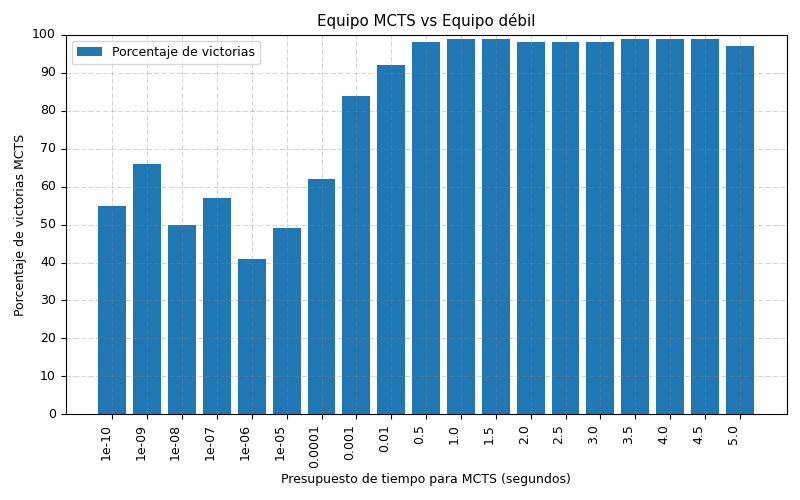
\includegraphics[scale=0.65]{graficas_experimentos/mcts_is_correct.png}}
        \caption{MCTS v.s. Greedy. MCTS vence en más del 90\% de los juegos con
        una décima de segundo de presupuesto de tiempo. Para cada presupuesto de
        tiempo se realizaron 100 juegos.}
        \label{MGA}
    \end{center}
\end{figure}

En la figura \ref{MGA} tenemos una gráfica del resultado de las simulaciones. En
el eje horizontal se muestra el presupuesto de tiempo que se le permitió
ejecutar a MCTS para cada tiro. Se corrieron múltiples simulaciones con
distintas configuraciones de MCTS de cien juegos cada una. Podemos observar que
muy rápidamente se llega a superar al equipo greedy. Con un presupuesto de una
milésima de segundo, la búsqueda en árbol logró vencer al jugador greedy en 80\%
de los juegos.

El desempeño observado nos indica que MCTS está calculando buenas jugadas y que
el módulo funciona correctamente.


\section{Búsqueda en cuadrícula}

Una vez que se ganó certeza sobre el correcto funcionamiento de la búsqueda en
árbol, la siguiente interrogante a resolver fue la elección de parámetros. El
algoritmo PIMC consta de dos parámetros a definir: el número de escenarios que
se generarán (n) y el presupuesto de tiempo (t) para buscar una acción óptima en
cada escenario usando MCTS.

Como punto de partida, se agregó como restricción que el tiempo total de
ejecución no debe exceder un segundo. Es decir, restringimos el espacio de
búsqueda a aquellas parejas de parámetros que satisfacen: 


\[nt = 1 \]

La métrica objetivo que se busca maximizar con la elección de parámetros es el
porcentaje de victorias de un equipo PIMC contra un equipo débil y un equipo
fuerte. Para el equipo débil se utilizaron los jugadores \textit{greedy} antes
descritos. Para el equipo fuerte se utilizó un jugador MCTS con conocimiento de
todas las fichas repartidas. Se justifica la elección del jugador fuerte
basándose en que un jugador humano experto tiene una gran habilidad para inferir
las fichas de los demás participantes. Además, posee una gran compenetración con
su compañero para poder cooperar armónicamente.

\begin{figure}[ht]
    \begin{center}
        \hbox{\hspace{-2em}
        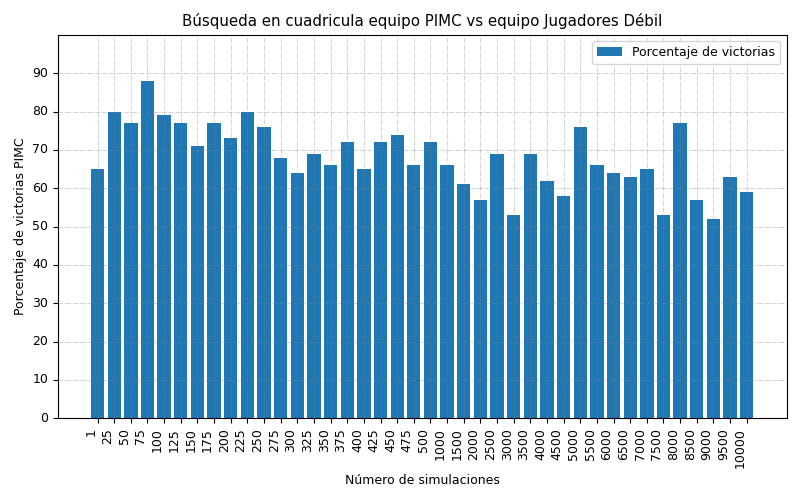
\includegraphics[scale=0.65]{graficas_experimentos/grid_search_vs_greedy.png}}
        \caption{Búsqueda en cuadrícula equipo PIMC vs equipo débil. Se muestran
        concatenados dos rangos. El rango 1-500 tiene saltos de 25 unidades. El
        rango 500 - 10,000 tiene saltos en 500 unidades. Para cada n, se eligió
        t tal que \(nt = 1\). Para cada configuración se simularon 100 juegos.}
        \label{GSW}
    \end{center}
\end{figure}

En la figura \ref{GSW} se muestran los resultados de los juegos entre PIMC y
greedy. Se puede observar que en el rango \( n \in  [25, 125] \) es donde PIMC
tiene mejor desempeño. También se observa que en el rango  \( n \in  [1000,
10000]\) el porcentaje de victorias disminuye y tiene mayor variabilidad
conforme cambia n.

\begin{figure}[ht]
    \begin{center}
        \hbox{\hspace{-2em}
        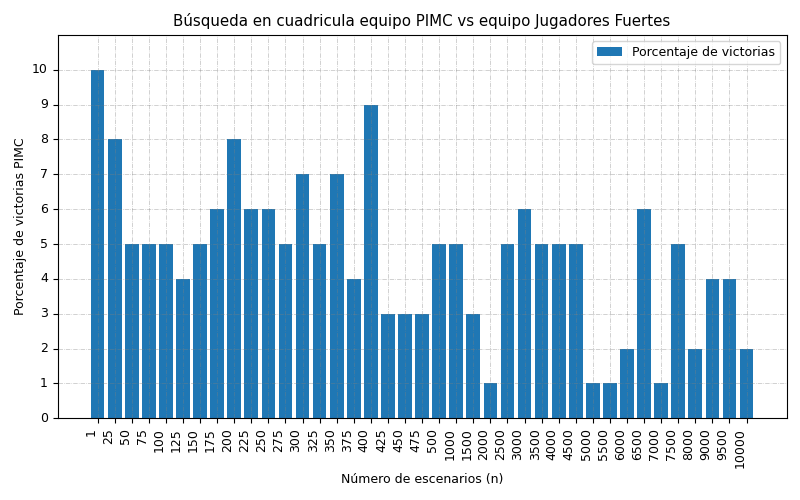
\includegraphics[scale=0.65]{graficas_experimentos/grid_search_vs_strong.png}}
        \caption{Búsqueda en cuadrícula equipo PIMC vs equipo fuerte. Se muestran
        concatenados dos rangos. El rango 1-500 tiene saltos de 25 unidades. El
        rango 500 - 10,000 tiene saltos en 500 unidades. Para cada n, se eligió
        t tal que \(nt = 1\). Para cada configuración se simularon 100 juegos.}
        \label{GSS}
    \end{center}
\end{figure}

En la figura \ref{GSS} se pueden observar los resultados de la búsqueda al jugar
contra un equipo fuerte. A diferencia de la figura \ref{GSW}, es menos clara una
tendencia en los datos. El mejor desempeño se logró cuando PIMC sólo tomó en
cuenta un escenario. Esta configuración de parámetros es un caso degenerado en
donde PIMC se convierte en MCTS aplicado a un escenario aleatorio de repartición
de fichas, por lo que se podría pensar que no es la elección más deseada de
parámetros. Aun así, parece apreciarse que en el rango \( n \in  [1, 400] \) el
desempeño del jugador es mejor que en el resto de las configuraciones.

\section{Desempeño del sistema}

El análisis anterior fue útil para elegir una combinación de parámetros . Se
eligieron los valores \(n^* = 75 \) y \( t^* = \frac{1}{75}\), los cuales
maximizaron el porcentaje de victorias en la figura \ref{GSW} y se encontraban
en la región de mejor desempeño de la figura \ref{GSS}. 

\begin{table}[!ht]
    \centering
    \caption{Estadísticas de 100 juegos. Equipo PIMC vs equipo greedy}
    \begin{tabular}{|l|l|}
    \hline
        Porcentaje de victorias PIMC & 88.0 \\ \hline
        Porcentaje de victorias greedy & 10.0 \\ \hline
        Porcentaje empates & 2.0 \\ \hline
        Porcentaje victorias sin juego cerrado PIMC & 65.0 \\ \hline
        Porcentaje victorias sin juego cerrado greedy & 6.0 \\ \hline
        Promedio pases por juego PIMC & 1.63 \\ \hline
        Promedio pases por juego greedy & 2.69 \\ \hline
    \end{tabular}
    \label{MINP}
\end{table}

Como se puede ver en la tabla \ref{MINP}, el sistema cumplió con el
requerimiento de porcentaje de victorias contra el jugador \textit{greedy} al
ganar en 88 \% de los juegos. En promedio, en cada juego hubo casi 3 turnos del
equipo \textit{greedy} en que el jugador no tenía ninguna ficha para bajar, un
turno más que el equipo PIMC . La estadística sugiere que el equipo PIMC estaba
haciendo buenas jugadas que obligaron al equipo contrincante a pasar más
seguido.

En dominó, un juego se cierra cuando ningún equipo puede bajar más fichas. El
ganador es el equipo cuyas fichas suman el menor número de puntos. En la tabla
\ref{MINP} se muestra que en 65 \% de los juegos PIMC ganó sin juego cerrado, es
decir, ganó por que uno de los miembros del equipo bajó todas sus fichas. Así,
en 23 \% de los casos, PIMC ganó por tener menor número de puntos.


Después de validar que un equipo de dos jugadores PIMC eran superiores a un
equipo \textit{greedy}, se decidió investigar cómo variaba el desempeño para
equipos mixtos.

\begin{table}[!ht]
    \centering
    \caption{Estadísticas de 100 juegos. Equipo PIMC con jugador fuerte vs equipo greedy}
    \begin{tabular}{|l|l|}
    \hline
        Porcentaje de victorias PIMC con jugador fuerte & 88.0 \\ \hline
        Porcentaje de victorias greedy & 12.0 \\ \hline
        Porcentaje empates & 0.0 \\ \hline
        Porcentaje victorias sin juego cerrado PIMC con jugador fuerte & 67.0 \\ \hline
        Porcentaje victorias sin juego cerrado greedy & 7.0 \\ \hline
        Promedio pases por juego PIMC con jugador fuerte & 1.61 \\ \hline
        Promedio pases por juego greedy & 2.74 \\ \hline
    \end{tabular}
    \label{MIXS}
\end{table}

En la tabla \ref{MIXS} se muestran las estadísticas de 100 juegos de un equipo
mixto compuesto de un jugador PIMC y un jugador fuerte. Se observa que en
general las estadísticas del equipo con jugador PIMC fueron similares al de la
tabla \ref{MINP}. Así, el equipo mixto mostró mantener un buen desempeño contra
el equipo \textit{greedy}.


\begin{table}[!ht]
    \centering
    \caption{Estadísticas de 100 juegos. Equipo PIMC con jugador greedy vs equipo greedy}
    \begin{tabular}{|l|l|}
    \hline
        Porcentaje de victorias PIMC con jugador greedy & 72.0 \\ \hline
        Porcentaje de victorias greedy & 25.0 \\ \hline
        Porcentaje empates & 3.0 \\ \hline
        Porcentaje victorias sin juego cerrado PIMC con jugador greedy & 59.0 \\ \hline
        Porcentaje victorias sin juego cerrado greedy & 11.0 \\ \hline
        Promedio pases por juego PIMC con jugador greedy & 1.87 \\ \hline
        Promedio pases por juego greedy & 2.81 \\ \hline
    \end{tabular}
    \label{MIXG}
\end{table}

En contraste, la tabla \ref{MIXG} muestra las estadísticas de un equipo
compuesto de un jugador PIMC y un jugador \textit{greedy} contra un equipo
\textit{greedy}. Aquí es visible una perdida en el desempeño, bajando más de 10
puntos en el porcentaje de victorias. También el porcentaje de pases por juego
aumentó ligeramente para el equipo mixto. Aun así, el equipo mixto superó el 70
\% de victorias, como se buscaba en las restricciones del sistema.
